\documentclass[12pt]{article}
\usepackage[letterpaper,left=4.9cm,right=1.9cm,top=3.1cm,bottom=2.3cm]{geometry} % Márgenes y demás
\usepackage[nswissgerman]{babel}

\usepackage[utf8]{inputenc}
\usepackage{pxfonts}
\usepackage{abstract}
\usepackage{parskip}
\usepackage{wasysym} % symbols
\usepackage{amssymb} % symbols
\usepackage{xcolor}
\usepackage[colorlinks=false]{hyperref}
%\usepackage{amsmath}
\usepackage{float}
\usepackage{graphicx}
\usepackage{fancyhdr}
\usepackage{titling}
\usepackage{hyperref}
\usepackage{svg}
\usepackage{caption}
\usepackage{titlesec}
\usepackage{apacite}
\usepackage[document]{ragged2e}
\usepackage[affil-sl]{authblk} 
\usepackage{mathptmx}  %Times new Roman 

\makeatletter


\renewcommand{\maketitle}{\bgroup\setlength{\parindent}{14pt}
\begin{flushleft}
  \textbf{\@title}
  \@author 
\end{flushleft}\egroup}

\makeatother

\pagestyle{fancy}
\fancyfoot[C]{}
\fancyfoot[R]{\thepage}
\renewcommand{\headrulewidth}{0pt}
\fancyhead{
  \fancyhead[R]{}
}




%%% Citaciones y año en negrilla
\renewcommand{\BAstyle}{\bfseries}
%%%%%%%%%%%%%%%%%%%%%%%%%%%%%%%%%%

%%%%%%% Número de volúmen en negrilla
\renewcommand{\APACjournalVolNumPages}[4]{%
  \Bem{#1}%             journal
  \ifx\@empty#2\@empty
  \else
    \unskip, \textbf{\Bem{#2}}%  volume
  \fi
  \ifx\@empty#3\@empty
  \else
    \unskip({#3})%      issue number
  \fi
  \ifx\@empty#4\@empty
  \else
    \unskip, {#4}%      pages
  \fi
}
%%%%%%%%%%%%%%%%%%%


%%%%% Nombres de los autores en negrilla
\renewcommand{\APACrefauthstyle}{\bfseries}
%%%%%%%%%%%%%%%%%%%%%%%%%%%%%%%%%%%%%%%%



%% Comandos modificados al estilo
\renewcommand\Affilfont{\fontsize{8}{8}}

%%Tamaño fuente filiación 

\definecolor{bluesrev}{HTML}{136f8b}

\renewcommand{\absnamepos}{flushleft}
\renewcommand{\abstractnamefont}{\fontsize{13}{13}\bfseries}
\renewcommand{\abstracttextfont}{\fontsize{9}{1}\justifying}

\titleformat*{\section}{\fontsize{13}{1}\bfseries\color{bluesrev}}

\titleformat{\subsection} 
	{\normalfont\itshape }{\makebox[30pt][l]{\thesubsection}}{0pt}{}

\captionsetup{justification   = raggedright,
              singlelinecheck = false}

\captionsetup{labelfont=bf}
\captionsetup{labelsep=period}


\renewcommand{\figurename}{Figura}


%%% ORCID  %%%

\usepackage{scalerel}
\usepackage{tikz}

\definecolor{orcidlogocol}{HTML}{A6CE39}

%%%%%%%%%%%%%%%%%%%


  

\setlength{\topskip}{0.5cm}
\setlength{\parindent}{0mm}

%\title{\fontsize{14}{14}\textbf{Sleep Cube - Diary} \\[0.2cm]
\title{\textcolor{gray}{\textbf{sleepCube - Report Document}\\[0.2cm]}}


\author[1]{\fontsize{9}{9} \textbf{Ugur Turhal}}
\author[2]{\textbf{Silvan Lenzlinger}}
\author[1]{\textbf{Berkan Kurt}}

\affil[1]{\fontsize{8}{8}\href{mailto:ugur.turhal@me.com}{ugur.turhal@me.com}}
\affil[2]{test}
\affil[3]{test}
\date{\today}                     
\setcounter{Maxaffil}{0}

\usepackage{listings}    

\definecolor{mygreen}{rgb}{0,0.6,0}
\definecolor{mygray}{rgb}{0.47,0.47,0.33}
\definecolor{myorange}{rgb}{0.8,0.4,0}
\definecolor{mywhite}{rgb}{0.98,0.98,0.98}
\definecolor{myblue}{rgb}{0.01,0.61,0.98}

\lstset{ %
  backgroundcolor=\color{mywhite},   
  basicstyle=\footnotesize,       
  breakatwhitespace=false,         
  breaklines=true,                 
  captionpos=b,                   
  commentstyle=\color{mygray},    
  deletekeywords={...},           
  escapeinside={\%*}{*)},          
  extendedchars=true,              
  frame=false,                    
  keepspaces=true,                 
  keywordstyle=\color{myorange},       
  language=C,                
  morekeywords={*,...},            
  numbers=left,                    
  numbersep=5pt,                   
  numberstyle=\tiny\color{mygray}, 
  rulecolor=\color{black},         
  rulesepcolor=\color{myblue},
  showspaces=false,                
  showstringspaces=false,          
  showtabs=false,                  
  stepnumber=2,                    
  stringstyle=\color{myorange},    
  tabsize=2,                       
  title=\lstname                   
}    



\begin{document}
\maketitle

\section{7.12.2021 - 18.12.2021 - Einkauf \& Testing}
\justifying
\subsection{Bestellung der Einzelteile} 
Die Bestellung der Einzelteile war nicht simpel. Es haben sich grössere Fragen eröffnet: Ist das Kupferkabel genug stark, aber auch nicht zu dick im Umfang, für unsere Konstruktion? Wie wollen wir das verlöten? Was wenn ein Teil defekt ist? Wie lange dauert die Lieferung? Wir haben die Bestellung in Tranchen erhalten. Die Reihe war wiefolgt: Distrilec, Distrilec, Amazon \& Reichelt zu dem Einkäufe am 18.12.2021. \par \subsection{Testing} Ugur hat die Bestellung überprüft: Die LEDs wurden einzeln getestet ob diese funktionieren oder nicht, siehe Bild \ref{Fig:leds}. Die Funktionalität des Multimeters wurde mit der Knopfdruckbatterie getestet. Unser Motto, \glqq lieber eine Komponente mehr\grqq\ hat sich bewährt, da ein Temperatur Sensor defekt geliefert wurde. Das wurde mittels einem Arduino getestet \& festgestellt. Ein DHT22 Sensor gab den gewünschten Output, der andere wurde nicht erkannt von dem Breadboard. Alle anderen Teile wurden auf Unversehrtheit überprüft, siehe Tabelle \ref{Tab:table1}.
\begin{table}[H]
\begin{center}
\begin{tabular}{l|l}
Komponente & Funktioniert \\ \hline
\hline
Rote LEDs   & Ja \\ \hline
Grüne LEDs   & Ja \\ \hline
DHT22   & Teilweise \\ \hline
Europlatine   & Ja \\ \hline
Kabel  & Ja  \\ \hline
Schrumpfschlauch & Ja \\ \hline
Stiftleiste   & Ja \\ \hline
Kupferkabel Cable  & Ja \\ \hline
100 OHM  & Ja \\ \hline
Flussmittel & Ja \\ \hline
Multimeter & Ja \\ \hline
\end{tabular}
\caption{Benötigte Komponenten}
\label{Tab:table1}
\end{center}
\end{table}
\begin{figure}[H]
\begin{center}
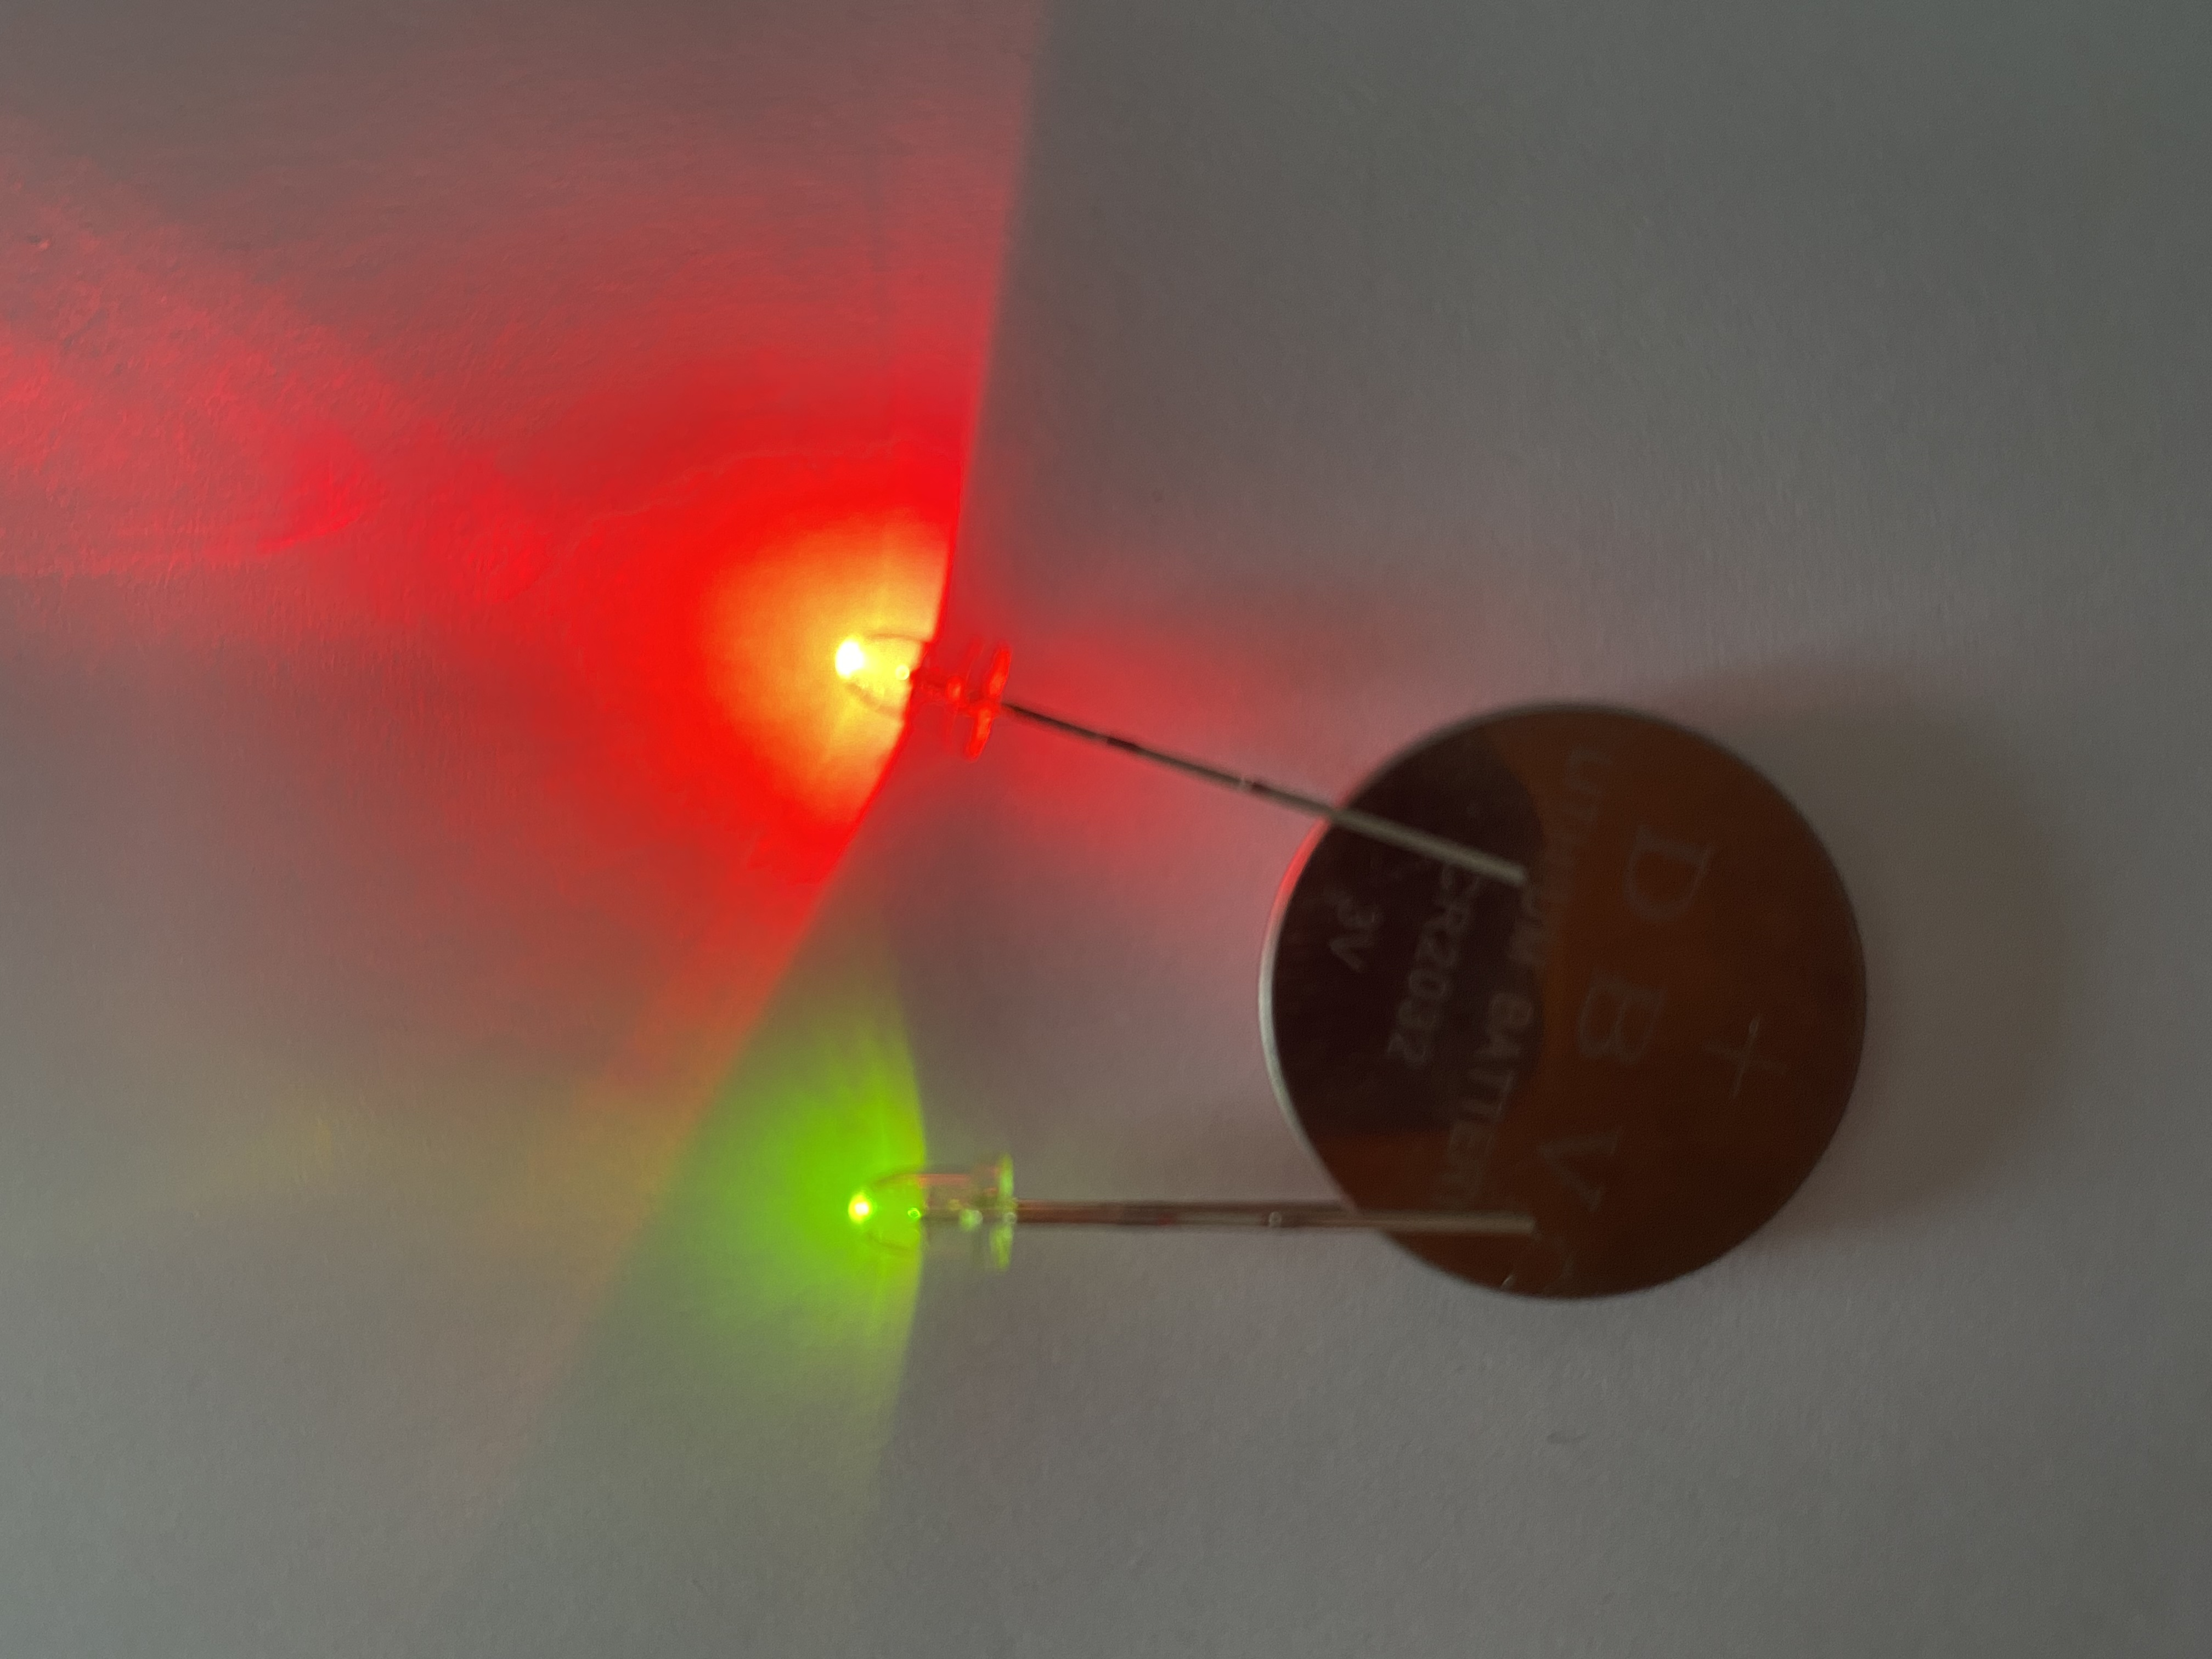
\includegraphics[width=0.5\textwidth]{pics/leds.jpeg}
\caption{LEDs mit Knopfdruckbatterie getestet}
\label{Fig:leds}
\end{center}
\end{figure}\par
Wir sind bereit, die nächsten Schritte vorzunehmen, diese Beinhalten: 
\begin{itemize}
\item simple Version mit Sensor und LEDs.
\item Die Anordnung der LEDs.
\item Lötumgang erlernen.
\end{itemize} Ugur beginnt ein simples Modell zu erfassen. Auch erhalten wir \underline{alle} nächste Woche von Sarah-Lia einen Crashkurs zum Umgang mit dem Lötkolben, Flussmittel, Lötzinn \& Schrumpfschlauch.
\section{Erstes Modell \& Einführung in das Löten}
\subsection{DHT22}
Als erstes muss die Library für DHT11/DHT22 hinzugefügt werden in der Arduino IDE. 
\begin{lstlisting}
#include "DHT.h" 
//Pin Nummer wo der Sensor angeschlossen ist               
#define DHTPIN 2
// Hier wird definiert was fuer ein Sensor ausgelesen wird.
#define DHTTYPE DHT11
\end{lstlisting}
\subsection{Einführung in das Löten}
\end{document}
